\documentclass{article}

\usepackage{graphicx}         % Pacote para usar os gráficos
\usepackage[utf8]{inputenc}		% Pacote para usar acentos


\begin{document}


% Vamos fazendo junto com eles
% DEVAGAR
% SÉRIO
% FAÇAM
% DEVAGAR

\section{Minha seção top} \label{sec:top}
  Vamos fazer o negócio aqui ~~ imagine um texto longo para encher linguiça ~~.

  % Dá pra fazer essa figura com o WIZARD do TeXStudio, assim não perdemos tanto tempo
  \begin{figure}[h]
    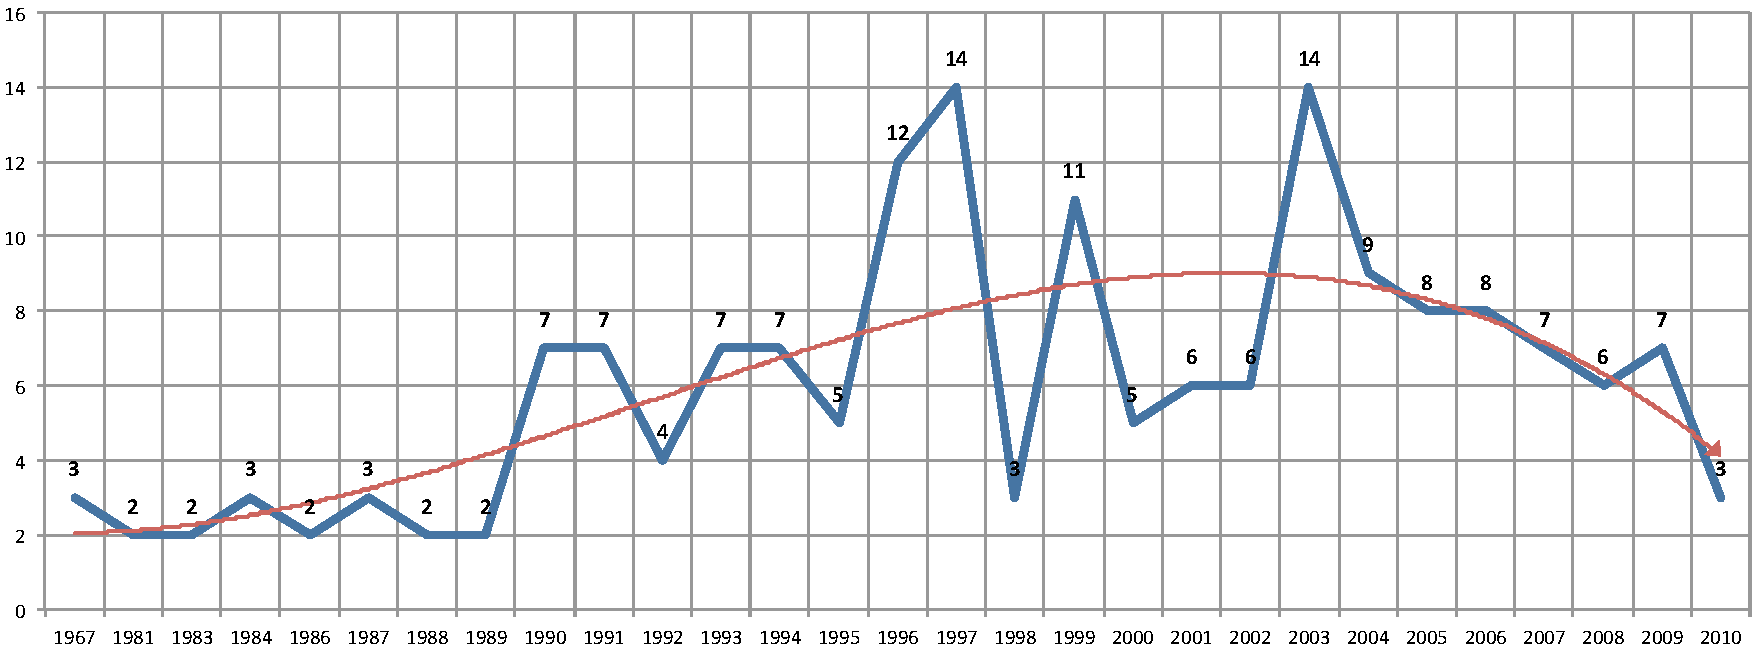
\includegraphics[scale=0.5]{abntex2-modelo-img-grafico}
    \caption{Minha figura top}
    \label{fig:top}
  \end{figure}

  Agora eu referencio essa figura acima como sendo Figura \ref{fig:top}. Legal, né?

  Observe essa belíssima tabela abaixo, nomeada como Tabela \ref{tab:top}. Linda, né?
  % Dá pra fazer essa tabela com o WIZARD do TeXStudio, assim não perdemos tanto tempo
  \begin{table}[h]
    \centering
    \begin{tabular}{| l | l |}
      \hline
      Bom & dia \\
      \hline
    \end{tabular}
    \label{tab:top}
    \caption{Minha tabela top}
  \end{table}

  \section{Seção 2 para exemplos legais}

  Conforme visto na Seção \ref{sec:top}, aprendemos a fazer referências!!!

  Agora eu vou adicionar uma nova tabela e referenciá-la como Tabela \ref{tab:informacao-importante}.
  % Dá pra fazer essa tabela com o WIZARD do TeXStudio, assim não perdemos tanto tempo

  \begin{table}[h]
	\centering
	\begin{tabular}{| l | l |}
		\hline
		Boa & noite \\
		\hline
	\end{tabular}
	\label{tab:informacao-importante}
	\caption{Minha tabela com informações importantes}
\end{table}

\end{document}
